\documentclass{beamer}

\usepackage[brazil]{babel}
\usepackage[T1]{fontenc}
\usepackage[utf8]{inputenc}

\usetheme{CambridgeUS}
\usecolortheme{seagull}
\setbeamertemplate{title page}[default][shadow=false]
\setbeamertemplate{headline}{}
\setbeamertemplate{itemize items}[triangle]
\setbeamertemplate{footline}[frame number]{}
\setbeamertemplate{navigation symbols}{}

\title{Esquemas de assinatura digital\\baseados em funções de resumo}
\subtitle{Aprimoramento de esquemas antigos}
\author{Gustavo Zambonin}
\institute{
  Universidade Federal de Santa Catarina \\
  Departamento de Informática e Estatística
}
\date{}

\newcommand{\concat}{\, \vert \vert \,}
\newcommand{\hash}[2][]{\mathcal{H}^{#1}(#2)}

\begin{document}

\begin{frame}[noframenumbering, plain]
  \titlepage
\end{frame}

\begin{frame}
  \frametitle{Esquemas introdutórios}
  \begin{itemize}
    \item Lamport-Diffie tem assinaturas e pares de chaves muito grandes
    \item Merkle (MSS) verifica um número limitado de assinaturas com sua
      chave pública, e não é eficiente de modo geral
    \item novos esquemas, mais eficientes e seguros
  \end{itemize}
\end{frame}

\begin{frame}
  \frametitle{Esquema de assinatura de Winternitz
    \cite{Bernstein:2008:PQC:1522375, Buchmann:2011:SWO:2026469.2026501}}
  \begin{itemize}
    \item aplica-se a função $\mathcal{H}$ repetidamente em uma entrada secreta
    \item número de iterações depende da mensagem a ser assinada
    \item parâmetro $w \in \mathbb{N}$ define o número de bits a serem
      assinados simultaneamente
    \item notação
    \begin{itemize}
      \item $\stackrel{\$}{\longleftarrow}$: `'gerado aleatoriamente de`'
      \item $\Delta^{(x_1, x_2)}$: $x_2$ palavras de tamanho $x_1$ compostas
        pelo alfabeto $\Delta$
      \item $\hash[x]{m} = \hash{\hash[x-1]{m}}, \hash[0]{m} = m$
    \end{itemize}
  \end{itemize}
\end{frame}

\begin{frame}
  \frametitle{Winternitz -- descrição do algoritmo}
  \begin{itemize}
    \item $\mathcal{G}$:
      $t_1 = \lceil \frac{n}{w} \rceil,
       t_2 = \lceil \frac{\lfloor log_2 t_1 \rfloor + 1 + w}{w} \rceil,
         t = t_1 + t_2$ \\

      \hspace{1.1em}
      $S_k = (y_{t - 1}, \dots, y_{0})
        \stackrel{\$}{\longleftarrow} \{0,1\}^{(n, t)}$ \\

      \hspace{1.1em}
      $P_k = (\hash[2^w - 1]{y_{t - 1}}, \dots, \hash[2^w - 1]{y_0})$

    \item $\mathcal{S}$:
      $\hash{m} \concat 0^*
        = (p_{t - 1}, \dots, p_{t - t_1}) \in \{0, 1\}^{(w, t_1)}$ \\

      \hspace{1.1em}
      $c = \sum_{i = t - t_1}^{t - 1} (2^w - p_i)$ \\

      \hspace{1.1em}
      $c \concat 0^* = (p_{t_2 - 1}, \dots, p_{0}) \in \{0, 1\}^{(w, t_2)}$ \\

      \hspace{1.1em}
      $\sigma = (\mathcal{H}^{p_{t - 1}}(y_{t - 1}),
        \dots, \mathcal{H}^{p_0}(y_0))$

    \item $\mathcal{V}$:
      $\forall \sigma_i \in \sigma,
        \hash[2^w - 1 - p_{i}]{\sigma_i} = P_{k_i}, 0 \leq i \leq t - 1$
  \end{itemize}
\end{frame}

\begin{frame}
  \frametitle{\emph{eXtended Merkle Signature Scheme} -- XMSS
    \cite{Buchmann:2011:XPF:2184003.2184011}}
  \begin{itemize}
    \item chave privada muda a cada assinatura
    \item necessidade apenas de $\mathcal{H}$ resistente à segunda pré-imagem
    \item encadeamento de árvores
  \end{itemize}

  \begin{figure}
    \centering
    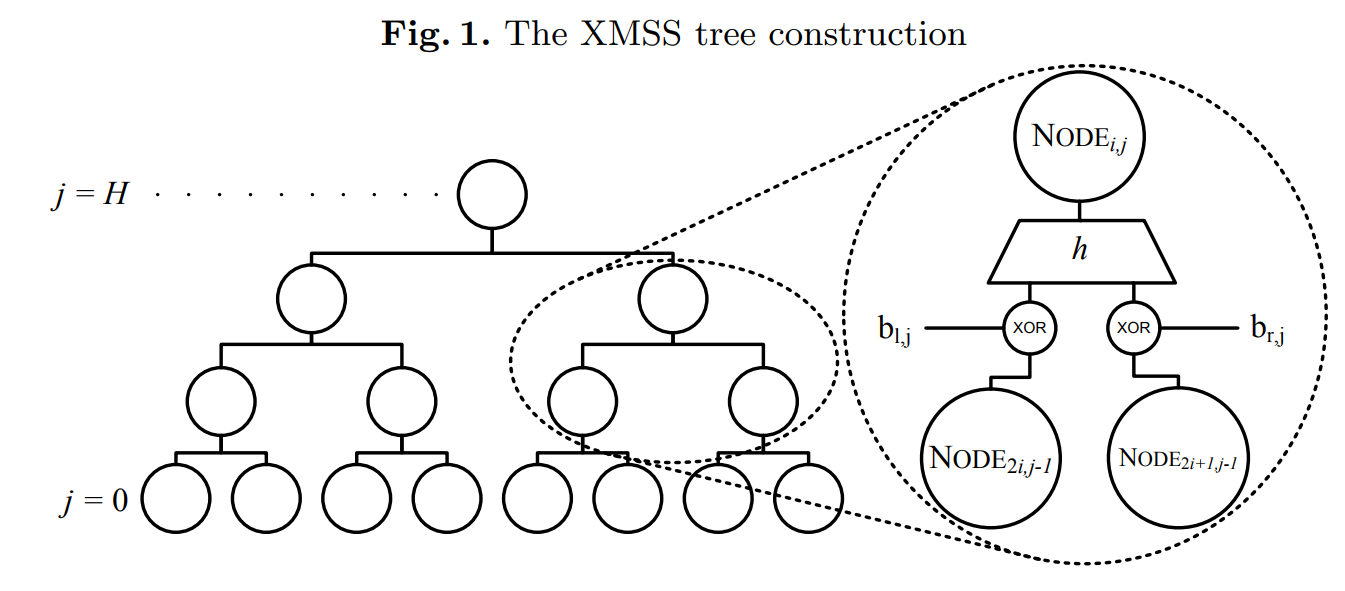
\includegraphics[scale=0.2]{xmss-example.png}
  \end{figure}
\end{frame}

\begin{frame}
  \frametitle{XMSS -- particularidades}
  \begin{itemize}
    \item máscaras de bits pseudo-aleatórias entre pais e filhos
    \item cada folha da árvore principal é uma L-tree
    \item folhas desta são os elementos de $P_k$ de Winternitz
  \end{itemize} \\

  \begin{itemize}
    \item $P_k$ contém as máscaras e a raiz da árvore
    \item $S_k$ contém a semente de um PRNG utilizado para gerar as $S_k$
      de Winternitz, e o índice da última assinatura feita
    \item $\mathcal{S}_i = (i, \sigma, A)$,
      onde $A$ é o caminho de autenticação
    \item verificação similar ao esquema de Merkle
  \end{itemize}
\end{frame}

\begin{frame}[allowframebreaks]
  \frametitle{Referências}
  \bibliography{\jobname}
  \bibliographystyle{abbrv}
\end{frame}

\end{document}
